\section{Metodología}
\label{sec:metodologia}

\subsection{Representación de las arquitecturas implementadas}

La Figura~\ref{fig:arquitecturas-av4} representa los tres diseños entrenados
desde cero. La entrada efectiva es una imagen RGB de $112\times112$ píxeles,
obtenida de los TFRecord de $224\times224$ mediante redimensionamiento bilineal
con antialias.

\begin{figure*}[p]
\centering
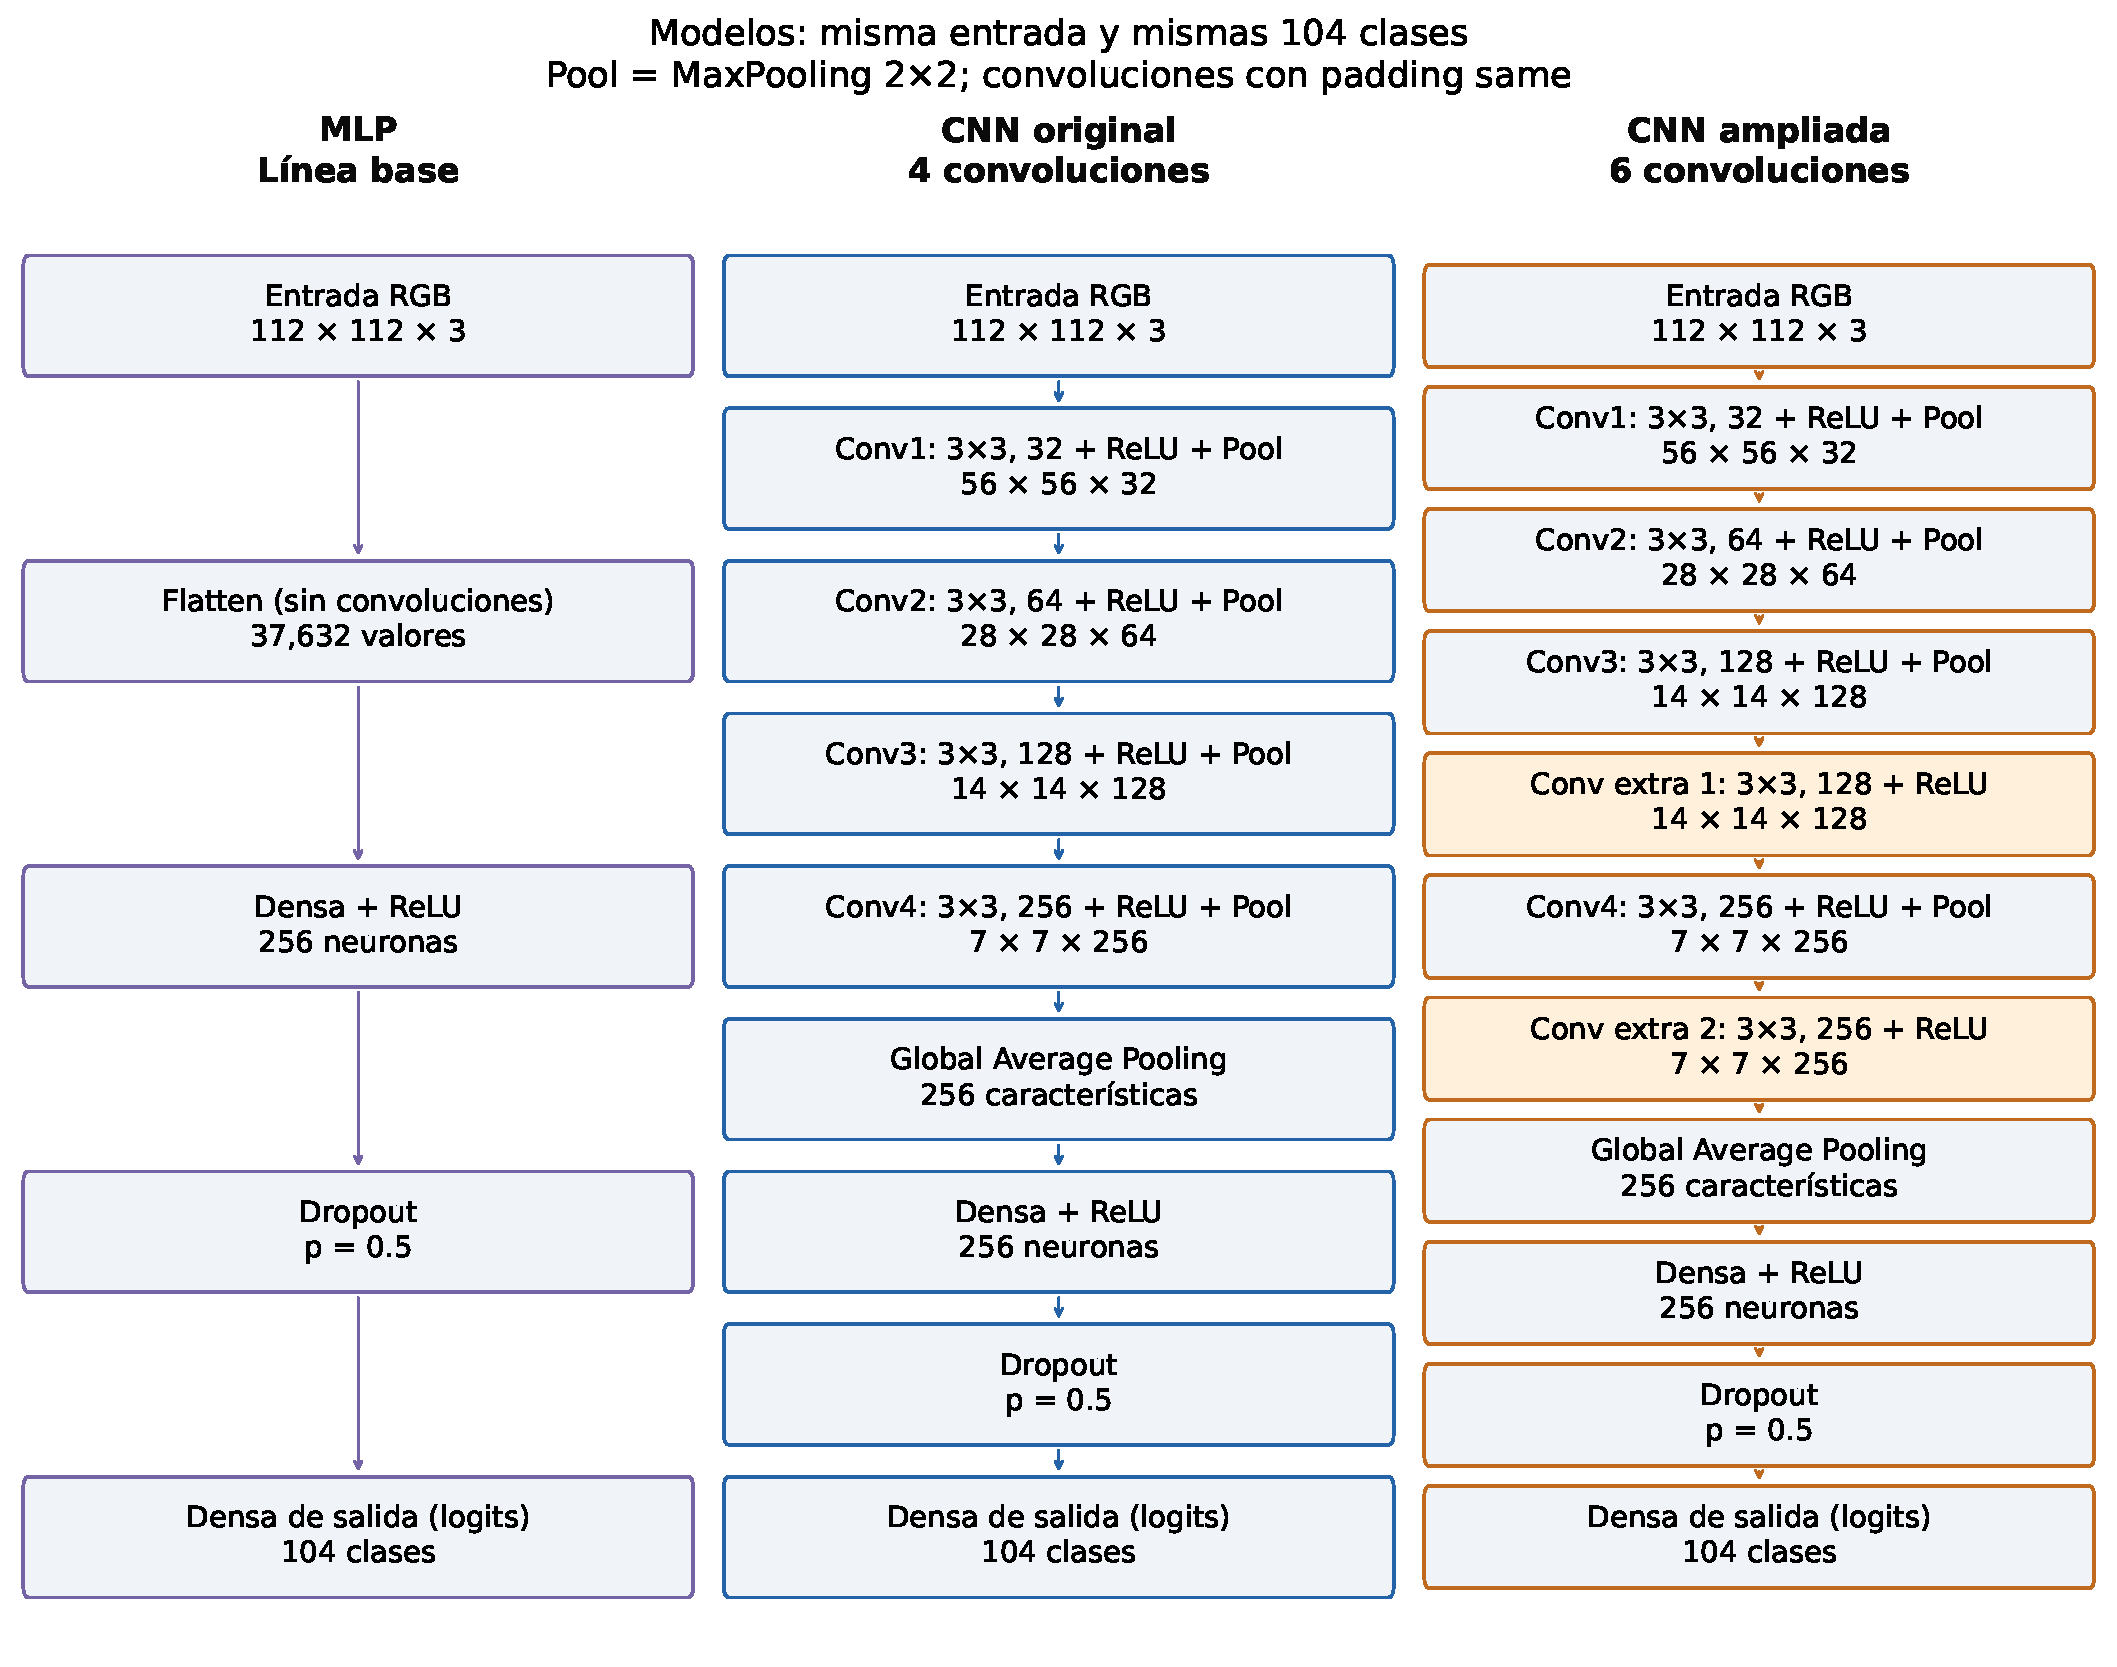
\includegraphics[width=\textwidth,height=0.85\textheight,keepaspectratio]{arquitecturas.pdf}
\caption{Representación de la red totalmente conectada de referencia, la CNN
original y la CNN con dos convoluciones adicionales. Las dimensiones corresponden
a las salidas de cada etapa; las capas adicionales se destacan en naranja.
La variante regularizada conserva la arquitectura de la CNN original.}
\label{fig:arquitecturas-av4}
\end{figure*}

La red \textbf{totalmente conectada de referencia} aplana los $112\times112\times3$
valores de entrada en un vector de 37,632 componentes. Aplica una capa densa de
256 unidades con ReLU, dropout \autocite{srivastava2014dropout} de 0.5 y una salida de 104 logits. No contiene
convoluciones ni pooling. Utiliza el mismo cargador, aumentos y ciclo de entrenamiento que la CNN.

La \textbf{CNN original} emplea cuatro convoluciones de $3\times3$, padding
\textit{same}, ReLU y 32, 64, 128 y 256 filtros. Cada convolución va seguida de
max pooling de $2\times2$. Las salidas de esos bloques son
$56\times56\times32$, $28\times28\times64$, $14\times14\times128$ y
$7\times7\times256$. Después aplica global average pooling (GAP), una capa densa
de 256 unidades con ReLU, dropout de 0.5 y 104 logits de salida.

La \textbf{CNN ampliada} agrega dos capas convolucionales ocultas: una de 128
filtros después del tercer pooling y otra de 256 después del cuarto. Ambas usan
kernel $3\times3$, padding \textit{same} y ReLU, sin pooling adicional. Por tanto,
esta versión tiene seis convoluciones. No se trata de dos capas densas nuevas.

La Tabla~\ref{tab:parametros} desglosa los parámetros por capa. En una
convolución de $3\times3$ con $C_{\text{in}}$ canales de entrada y
$C_{\text{out}}$ filtros hay $(9\,C_{\text{in}}+1)\,C_{\text{out}}$ parámetros, y
en una capa densa $(n_{\text{in}}+1)\,n_{\text{out}}$; el pooling no tiene
parámetros. En la CNN original, el 61\% de los parámetros está en la última
convolución, y las dos capas extra de la ampliada (737,664 parámetros) más que
duplican el total. En la MLP, en cambio, la primera capa densa concentra
$(37{,}632+1)\times256 = 9{,}634{,}048$ parámetros, el 99.7\% del total.

\begin{table}[htbp]
\centering
\caption{Parámetros entrenables por capa de las dos CNN.}
\label{tab:parametros}
\small
\setlength{\tabcolsep}{4pt}
\begin{tabular}{llrr}
\toprule
Capa & Salida & Original & Ampliada \\
\midrule
Conv 32 & $112\times112\times32$ & 896 & 896 \\
Conv 64 & $56\times56\times64$ & 18,496 & 18,496 \\
Conv 128 & $28\times28\times128$ & 73,856 & 73,856 \\
Conv 128 (extra) & $14\times14\times128$ & -- & 147,584 \\
Conv 256 & $14\times14\times256$ & 295,168 & 295,168 \\
Conv 256 (extra) & $7\times7\times256$ & -- & 590,080 \\
Densa 256 & 256 & 65,792 & 65,792 \\
Salida & 104 & 26,728 & 26,728 \\
\midrule
Total & & 480,936 & 1,218,600 \\
\bottomrule
\end{tabular}
\par\smallskip
\parbox{0.95\columnwidth}{\footnotesize Todas las convoluciones son de $3\times3$; la densa va después del GAP. Cada convolución va seguida de max pooling de $2\times2$ (sin parámetros), salvo las dos extra. La salida indicada es la de la convolución, antes del pooling.}
\end{table}

La convolución comparte los pesos del filtro entre posiciones y analiza
vecindarios de píxeles. Así puede aprender bordes, texturas y partes de pétalos
antes de combinarlos. Una capa densa sobre píxeles aplanados asigna pesos
independientes a cada posición y no impone esta estructura local. Esta diferencia
motiva la comparación, pero la mejora debe comprobarse con las métricas.

\subsection{Preprocesamiento y aumento de datos}

Se decodifica cada JPEG como RGB, se convierten sus valores a float32, se
normalizan mediante $x_{\mathrm{norm}}=x/255$ y se redimensionan a $112\times112$.
Las etiquetas son enteros entre 0 y 103. Se mantiene la separación de archivos
original entre entrenamiento y validación, sin incorporar imágenes de validación
al entrenamiento.

Solo en entrenamiento se aplican volteo horizontal, rotación aleatoria de factor
0.05, zoom de 0.1 y contraste de 0.1. Los valores resultantes se recortan a $[0,1]$.
Los aumentos se calculan después de la caché y del mezclado, por lo que cambian
entre épocas. La validación usa imágenes deterministas sin aumentos.

\subsection{Pérdida y actualización de parámetros}

Los modelos producen 104 logits $z_k$. La entropía cruzada se calcula directamente
sobre ellos, sin añadir una segunda softmax a la pérdida:
\begin{equation}
L=-\log\left(\frac{\exp(z_c)}{\sum_{k=1}^{104}\exp(z_k)}\right),
\end{equation}
donde $c$ es la clase verdadera. Para visualizar la confianza se transforma la
salida mediante softmax; esta confianza no constituye una evaluación de calibración.

Todas las redes se optimizan con AdamW \autocite{loshchilov2019adamw}
(decaimiento de pesos desacoplado de 0.01, sin aplicarlo a los sesgos) y una
tasa inicial de $10^{-3}$ que se reduce a la mitad cuando la pérdida de
validación no mejora en dos épocas, hasta $10^{-5}$. La MLP es la excepción en
la tasa: usa $10^{-4}$ (mínimo $10^{-6}$), porque en el Avance~4 un primer
intento con $10^{-3}$ colapsó a predecir una sola clase. Todos los modelos usan
lotes de 64 imágenes y se entrenan con TensorFlow~2.18 sobre la GPU de una Mac
M4 (\texttt{tensorflow-metal}).

\subsection{Pesos por clase}
\label{sec:pesos}

Para contrarrestar el desbalance (Sección~\ref{sec:desbalance}), una variante
pondera la pérdida de cada imagen según su clase \autocite{he2009imbalanced}:
\begin{equation}
w_c = \frac{N}{K\,n_c},
\end{equation}
donde $N=12{,}753$ es el total de imágenes, $K=104$ el número de clases y $n_c$
las imágenes de la clase $c$. Una clase de tamaño promedio recibe peso 1; las
clases de 18 imágenes reciben 6.8 y \emph{iris} (782) recibe 0.16. Como
$\sum_c w_c n_c = N$, la escala total de la pérdida no cambia.
